\section{ShopChain}
    \subsection{Home}
    All'arrivo sulla piattaforma ShopChain l'utente si ritroverà nella pagina Home,
    dalla quale potrà scegliere se pagare completamente un ordine (o creare una MoneyBox per lo stesso),
    oppure visualizzare lo storico delle transazioni effettuate da e verso di lui sulla nostra piattaforma.
    In questa sezione viene descritta passo per passo il primo caso, ossia il pagamento di un ordine sulla piattaforma: 
    per procedere l'utente cliccherà sul bottone contrassegnato come "Simula Pagamento".

    %immagine della pagina home con il bottone evidenziato

    \subsection{Transazioni}


        \subsubsection{Dettagli della transazione}

        Dopo aver cliccato il bottone, all'utente verrà presentato il riepilogo dell'ordine, e verra messa a disposizione la possibilità
        di pagare interamente l'ordine o di creare una MoneyBox per lo stesso.

        %immagine pagina dettagli transazione

        \subsubsection{Visualizzazione Transazioni}

        Tornando alla pagina Home, rimangono due bottoni nel menù di sinistra: "Your Transactions" e "Inbound Transactions".
        Cliccando su di essi si apriranno, rispettivamente, le pagine per visualizzare le transazioni in uscita dal proprio account e quelle in entrata.


            \paragraph{Transazioni in uscita}

            \begin{figure}[H]
                \centering
                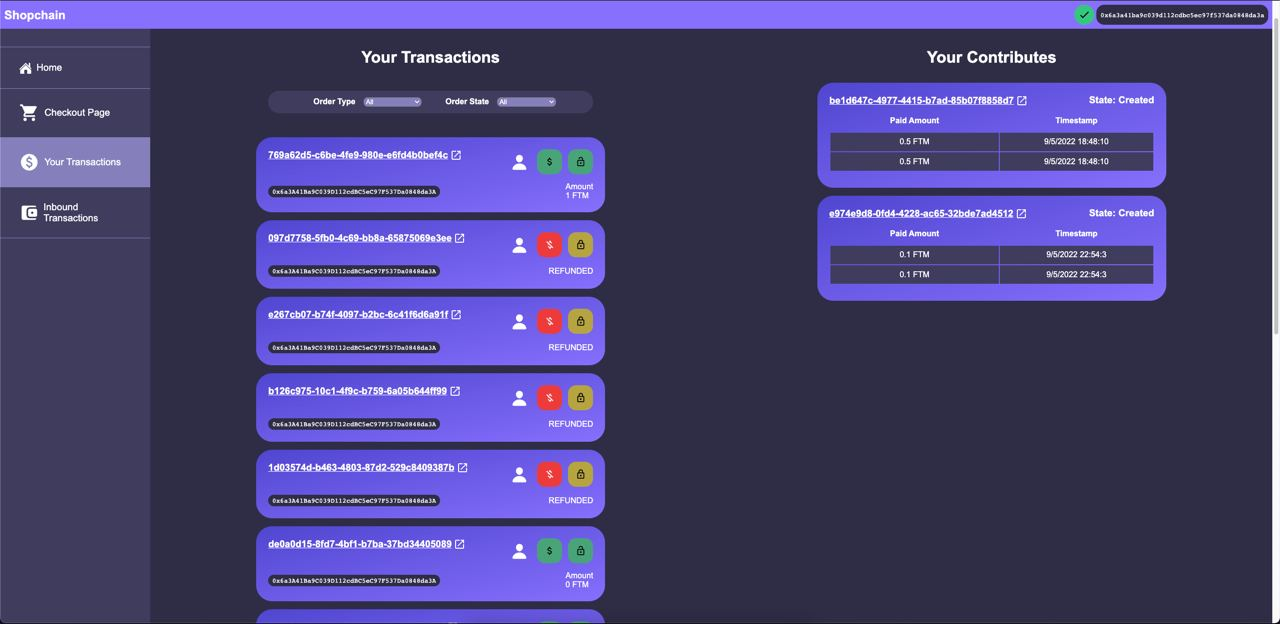
\includegraphics[scale=0.4]{immagini/transactionview.jpg}
                \caption{La vista delle transazioni in uscita}
            \end{figure}

            La pagina delle transazioni in uscita, "Your Transactions", è divisa in due sezioni:
            \begin{itemize}
                \item Yuor Transactions: in questa sezione sono riportati gli ordini \textbf{creati} dall'utente;
                \item Your Contributions: in questa sezione sono riportati gli ordini di tipo MoneyBox a cui l'utente ha pertecipato.
            \end{itemize}

            \paragraph{Transazioni in entrata}

            \begin{figure}[H]
                \centering
                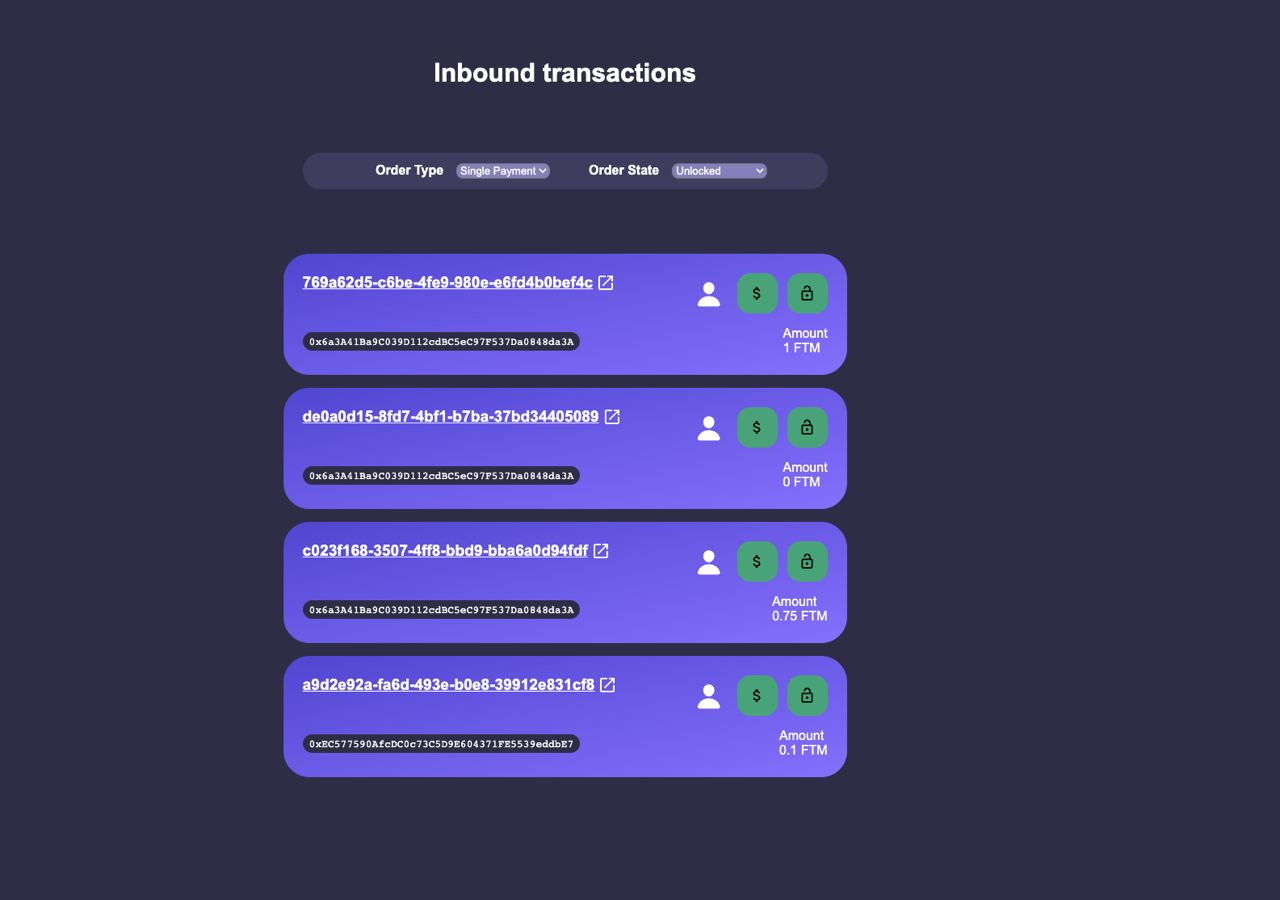
\includegraphics[scale=0.4]{immagini/inboundtransactions.jpg}
                \caption{La vista delle transazioni in entrata}
            \end{figure}

            Viceversa, la pagine delle transazioni in entrata, "Inbound Transactions", mostra solo una sezione con le transazioni effettuate verso il wallet dell'utente.

            \paragraph{Ordinamento transazioni}

            L'applicazione offre la possibilità di ordinare l'elenco delle transazioni in due possibili modalità, combinabili tra loro: 
            "Order Type", il tipo dell'ordine, e "Order State", lo stato corrente dell'ordine.
            La scelta è effettuata tramite un apposito menu a tendina.

            \begin{figure}[H]
                \centering
                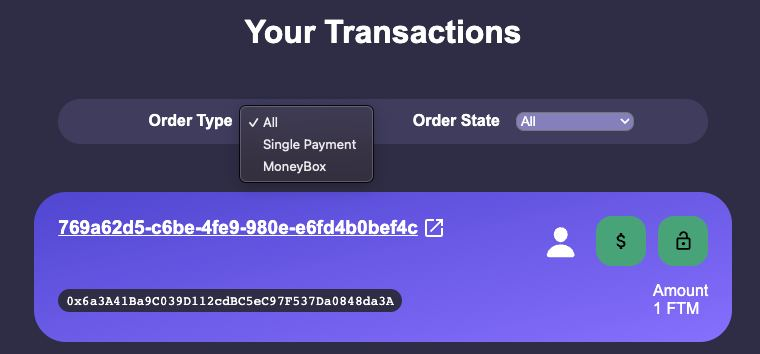
\includegraphics[scale=0.4]{immagini/ordertype.jpg}
             \caption{Menu per la scelta del tipo di ordine}
            \end{figure}

            Il tipo di ordine potrà essere:
            \begin{itemize}
                \item All: tutti i tipi di ordine;
                \item Single Payment: pagamento singolo;
                \item MoneyBox: pagamento creato come MoneyBox dall'utente.
            \end{itemize}

            \begin{figure}[H]
                \centering
                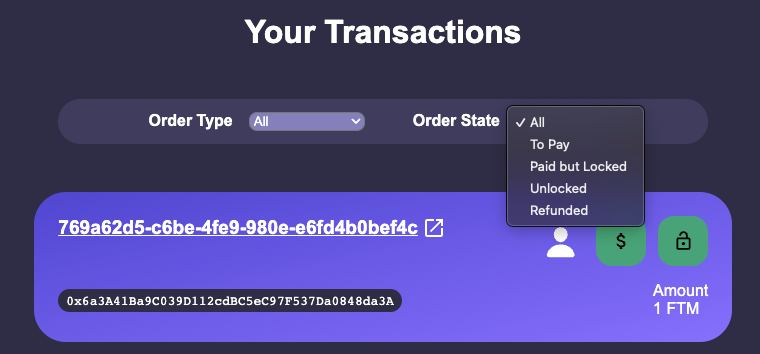
\includegraphics[scale=0.4]{immagini/orderstate.jpg}
                \caption{Menu per la scelta dello stato dell'ordine}
            \end{figure}

            Lo stato dell'ordine invece:
            \begin{itemize}
             \item All: tutti i tipi di stato;
                \item To Pay: il pagamento deve ancora essere completato;
                \item Paid but Locked: il pagamento è stato effettuato interamente, ma non ancora sbloccato;
                \item Unlocked: il pagamento è stato effettuato e sbloccato;
                \item Refunded: il pagamento è stato rimborsato.
            \end{itemize}

            L'ordinamento delle transazioni è disponibile sia per le transazioni in entrata che per quelle in uscita, e funziona in identico modo in entrambe le pagine.

            \paragraph{Transazione in dettaglio}

            \begin{figure}[H]
                \centering
                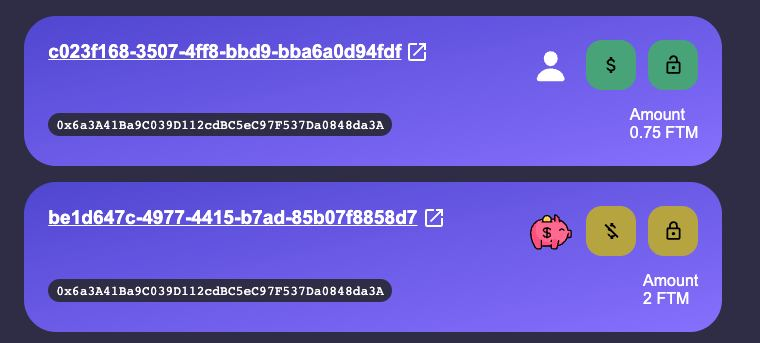
\includegraphics[scale=0.4]{immagini/transactionsmall.jpg}
                \caption{Due esempi di transazione nella lista "Your Transactions"}
            \end{figure}

            In dettaglio, le transazioni nelle liste sopracitate presentano all'utente le proprie informazioni più importanti.

            \begin{itemize}
                \item l'id univoco del pagamento, cliccabile, che rimanda alla pagina di riepilogo dell'ordine, mostrata nella sezione ??;
                \item l'indirizzo wallet dell'utente;
                \item un'icona per identificare il tipo di pagamento, singolo o MoneyBox;
                \item un'icona a forma di simbolo del dollaro per mostrare visivamente se la cifra richiesta è stata pagata interamente o meno;
                \item un'icona a forma di lucchetto per mostrate visivamente lo stato del pagamento;
                \item l'ammontare in FTM pagato.
            \end{itemize}

            L'icona di identificazione può assumere due forme: un icona di un uomo per il pagamento singolo, e l'icona di un maialino per il pagamento MoneyBox.

            \begin{figure}[H]
                \centering
                \begin{minipage}{0.45\textwidth}
                    \centering
                    
\includegraphics[scale=1]{immagini/uomo.jpg} 
                    \caption{Icona pagamento singolo}
                \end{minipage}\hfill
                \begin{minipage}{0.45\textwidth}
                 \centering
                    
\includegraphics[scale=1]{immagini/piggy.jpg} 
                    \caption{Icona pagamento MoneyBox}
                \end{minipage}
            \end{figure}

            L'icona di stato dell'ammontare pagato può assumere i seguenti colori: \textbf{verde}, se l'ammontare richiesto è stato raggiunto, o \textbf{giallo} nel caso sia ancora da raggiungere.\\

            L'icona di stato del pagamento avrà un colore diverso a seconda dello stato corrente del pagamento: \textbf{verde} per i pagamenti effettuati e sbloccati, 
            \textbf{giallo} per i pagamenti completati non ancora sbloccati o non ancora interi, \textbf{rosso} per i pagamenti rimborsati.

